\subsubsection{Pemodelan, Penyimpanan, dan \textit{Indexing} Data Smart Contracts}

% jadi bahas alternatif dulu, misal yang terpilih eth2dgraph
% lalu bahas schema yang dipakainya gimana, yang base nya apa aja secara singkat, dan yang mau ditambahinnya apa, berdasarkan apa
% Jadiin dua subheading

\begin{figure}[ht]
	\centering
	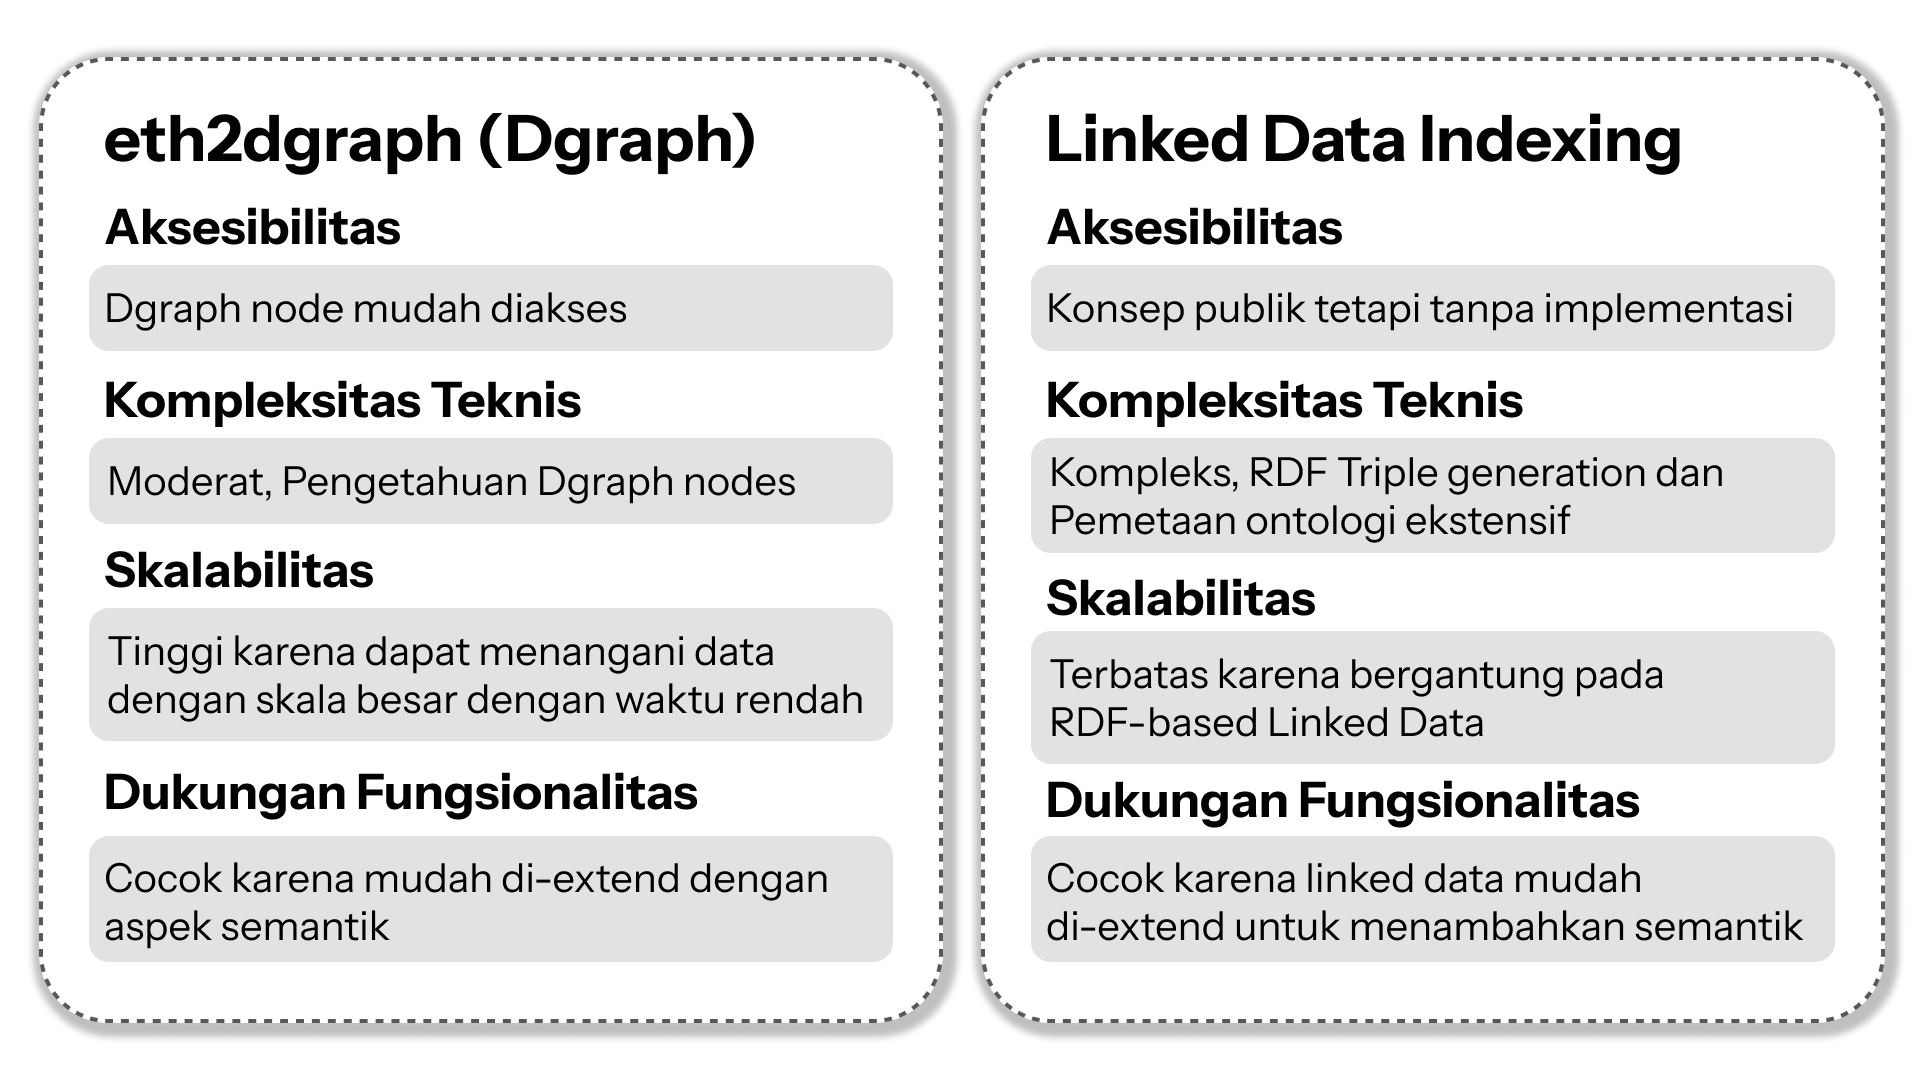
\includegraphics[width=0.9\textwidth]{resources/chapter-3/pemodelan-1.png}
	\caption{Perbandingan alternatif pemodelan, penyimpanan, dan \textit{indexing} data Smart Contracts}
	\label{image:pemodelan-1}
\end{figure}

\begin{figure}[ht]
	\centering
	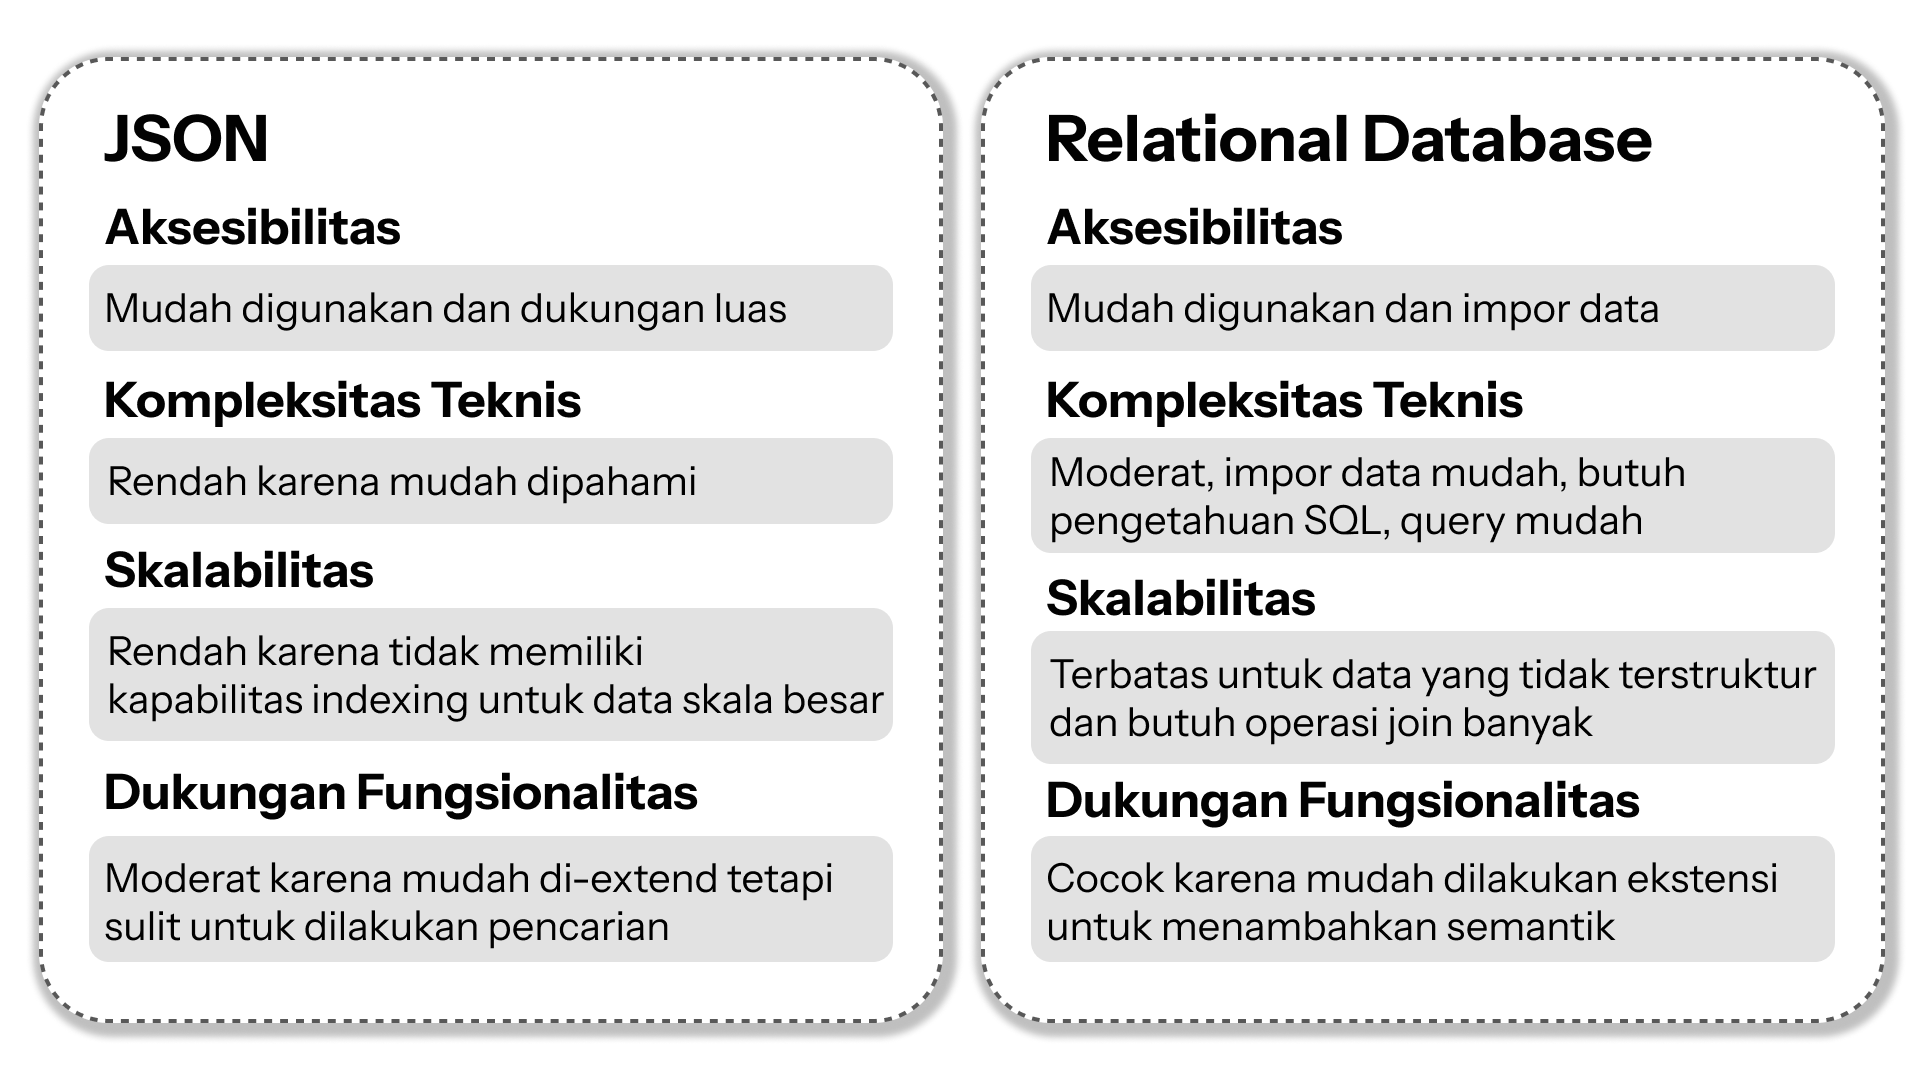
\includegraphics[width=0.9\textwidth]{resources/chapter-3/pemodelan-2.png}
	\caption{Perbandingan alternatif pemodelan, penyimpanan, dan \textit{indexing} data Smart Contracts}
	\label{image:pemodelan-2}
\end{figure}

Data yang diekstrak dari Blockchain Ethereum perlu dimodelkan, disimpan, dan dilakukan \textit{indexing} agar dapat diakses dengan efisien. Secara fungsional, untuk pemodelan, dibutuhkan ekstensibilitas yang baik untuk model, sehingga dapat menampung data yang lebih banyak dan lebih kompleks. Untuk penyimpanan, dibutuhkan skalabilitas yang baik untuk menyimpan data yang besar, serta dukungan untuk melakukan query dengan efisien. Untuk \textit{indexing}, dibutuhkan kemampuan untuk melakukan query dengan cepat dan efisien.

Gambar \ref{image:pemodelan-1} dan \ref{image:pemodelan-2} menunjukkan rangkuman perbandingan berbagai alternatif pemodelan, penyimpanan, dan \textit{indexing} data Smart Contracts. Secara rinci, berikut adalah analisis dari masing-masing alternatif:

\begin{enumerate}
	\item \textbf{eth2dgraph (Dgraph)} \parencite{aimar2023extraction}: Riset ini tidak hanya mengekstrak data, tetapi juga menyediakan solusi terpadu untuk pemodelan, indexing, dan penyimpanan dengan memanfaatkan Dgraph. Keunggulannya terletak pada skalabilitas tinggi dan efisiensi query, serta kemudahan akses dan eksekusi secara lokal. Meskipun memerlukan pemahaman dasar mengenai \textit{node} dan pemodelan graf, dokumentasi yang lengkap dan komunitas aktif membuat teknologi ini lebih mudah diaplikasikan. Format Dgraph juga mudah di-\textit{extend} untuk menambahkan aspek semantik yang mendukung pencarian Smart Contracts.

	\item \textbf{Linked Data Indexing of Distributed Ledgers (Linked Data)} \parencite{third2017linked}: Pendekatan riset ini bersifat publik namun tidak menyediakan implementasi open source. Metodenya membutuhkan pemetaan ontologi secara ekstensif dan generasi RDF triple yang kompleks, dengan dukungan tools atau framework yang minim. Selain itu, skalabilitasnya terbatas karena bergantung pada Linked Data berbasis RDF, meskipun format tersebut dapat dengan mudah di-\textit{extend} untuk menambahkan aspek semantik guna mendukung pencarian Smart Contracts.

	\item \textbf{JSON}: JSON menawarkan kemudahan penggunaan dan dukungan luas di berbagai bahasa pemrograman. Namun, meskipun sederhana dan mudah dikembangkan, JSON tidak mendukung indexing secara efisien untuk data besar, sehingga kurang ideal untuk sistem yang perlu menangani volume data tinggi.

	\item \textbf{Relational Database (SQL)}: Sistem basis data relasional dengan SQL unggul dalam indexing dan query yang efisien untuk data besar. Walaupun demikian, model relasional ini memiliki keterbatasan dalam fleksibilitas dan skalabilitas untuk data yang tidak terstruktur atau semi-terstruktur. Dengan pengetahuan dasar mengenai basis data relasional dan SQL, sistem ini dapat di-\textit{extend} melalui penambahan aspek semantik untuk memudahkan pencarian Smart Contracts.
\end{enumerate}